\documentclass[12pt, letterpaper, twoside]{article}
\usepackage[margin=2.50cm]{geometry} % Makes the Margins not stupid
\usepackage{bm} % for making bold equation variables
\usepackage{graphicx} % for placing images
\usepackage{float} % for making figure stay in place
\usepackage{amssymb} % for \lessapprox symbol
\usepackage{amsmath} % because using math and \text command in math mode
\usepackage[numbers]{natbib}
%-----------Pictures------------
\usepackage{graphicx}
\graphicspath{{./images/}}
\usepackage{wrapfig}
\usepackage[font=footnotesize,skip=0pt]{caption}

\title{Derivation of Continuity Equation in Spherical Coordinates}
\author{James Wright}
\date{2019-01-21}

\begin{document}
\maketitle

\begin{figure}[h]
    \centering
    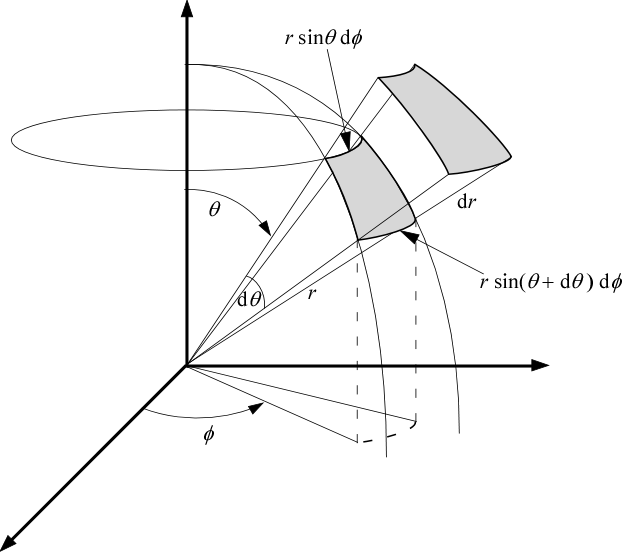
\includegraphics[width=0.6\textwidth]{images/control-volume-spherical.png}
    \caption{The control volume in spherical coordinates.}
    \label{fig:controlvolume}
\end{figure}

\section{Overview}

This document goes over the derivation of the continuity equation in spherical coordinates. It is assumed that the reader is already knowledgeable as to the nature of spherical coordinate systems.

The base equation that will be used is thus:

\begin{equation}
    \frac{\partial m}{\partial t}
\end{equation}

\end{document}